\section{Aufgabenstellung} 
\begin{frame}
  \frametitle{Personal Tutoring Service} 
	\begin{block}{\textbf{Projektdefinition}}
	  {\small Design und Implementierung einer webbasierten Anwendung um Personen 
	  zu helfen einen Tutor zu finden, sowie das anbieten der Dienste von Tutoren.}
	\end{block}
\end{frame}

\section{Projektleitung} 
\subsection{Teambildung}

\begin{frame} 
  \frametitle{Teambildung}
  \begin{block}{Herausforderungen}
    \begin{itemize}
      \item Sehr große Gruppe aus 12 Studenten
      \item Sechs Studenten ohne Vorkenntnisse in Web-Technologien
      \item Geringe Projekterfahrung unter allen Studenten
      \item Koordination
      \item Kommunikation
      \item Gemeinsames Entwickeln
      \item Enger Zeitplan
    \end{itemize}
  \end{block}
\end{frame}

\begin{frame} 
  \frametitle{Erste Maßnahmen}
    \begin{itemize}
      \item Feststellen vorhandener Fähigkeiten
      \item Bilden von Gruppen
      \begin{itemize}
        \item Front-End
        \item Back-End
        \item Content
      \end{itemize}
      \item Erstellen eines Terminplan
      \item Einführung einheitlichen Werkzeugen
      \item Vergabe von ``Lernaufgaben''
    \end{itemize}
\end{frame}

\subsection{Werkzeuge} 
\subsubsection{Git / Git-Hub}

\begin{frame} 
  \frametitle{Quellcodeverwaltung}
  \begin{block}{Git}
   Freie Software zur verteilten Versionsverwaltung von Dateien. 
   Ursprünglich zur Quellcode-Verwaltung des Linux-Kernels entwickelt.
  \end{block}
  Vorteile für das Projekt:
    \begin{itemize}
      \item Versionsverwaltung
      \item Nicht lineare Entwicklung möglich
      \item Synchronisation des Quellcodes via Git-Hub
    \end{itemize}
\end{frame}

\subsubsection{Dropbox}
\begin{frame} 
  \frametitle{Datenaustausch}
  \begin{block}{Dropbox}
    Online Cloud-Service zum transparenten Austausch von Daten.
  \end{block}
  Verwendung im Projekt:
    \begin{itemize}
      \item Austausch großer Daten
      \item Ablage von nicht produktiven Daten
      \begin{itemize}
        \item Protokolle
        \item Dokumente
        \item Referenzen
      \end{itemize}
    \end{itemize}
\end{frame}

\subsubsection{Kanban}

\begin{frame} 
  \frametitle{Aufgabenkoordination}
  \begin{block}{Kanban}
     Vorgehensmodell zur Softwareentwicklung.
     Visualisiert Aufgaben und Status der Teammitglieder.
  \end{block}
    \begin{figure}[htbp]
      \centering
        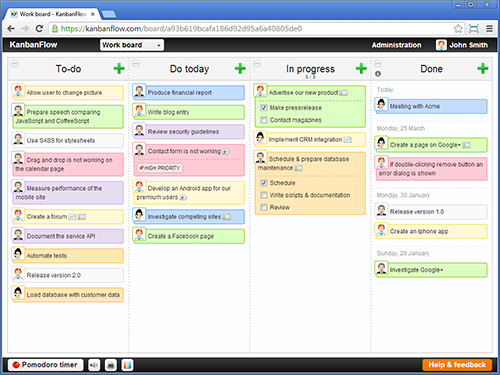
\includegraphics[width=0.45\textwidth]{./chapters/Kanban.png}
        \caption{KanbanFlow}
        \label{fig:Kanban}
   \end{figure}
\end{frame}


\subsection{Teamleitung}

\begin{frame} 
  \frametitle{Teamleitung}
  Aufgaben:
    \begin{itemize}
      \item Verteilung von Aufgabenpaketen
      \item Flexible Gruppengestaltung je nach Arbeitslast
      \item Kontrolle von Aufgaben
      \item Review von Sourcecode
      \item Motivation der Gruppenmitglieder
      \item Hilfestellung bei Programmierschwierigkeiten (Front-End)
    \end{itemize}
\end{frame}
